\documentclass{article}
\usepackage[top=1in, bottom=1in, left=1in, right=1in]{geometry}
% \usepackage{fullpage, fancyhdr}
\usepackage{fullpage}
\usepackage{float}
\usepackage{mathtools}
\usepackage{caption}
\usepackage{subcaption}
\usepackage{portland}
\usepackage{graphicx}
%\usepackage{setspace}
\setlength{\topmargin}{0.0in}
\setlength{\headheight}{0.5in}
\setlength{\headsep}{0in}
\setlength{\footskip}{9pt}


% \pagestyle{fancyplain}
\pagestyle{myheadings}
\voffset=-0.50in
\topmargin=0.00in 
\headsep=0.25in 
\evensidemargin=0in 
\oddsidemargin=0in 
\textwidth=6.6in 
\textheight=10.0in 

\renewcommand{\topfraction}{0.9}	% max fraction of floats at top
\renewcommand{\bottomfraction}{0.8}	% max fraction of floats at bottom
%   Parameters for TEXT pages (not float pages):
\setcounter{topnumber}{2}
\setcounter{bottomnumber}{2}
\setcounter{totalnumber}{4}     % 2 may work better
\setcounter{dbltopnumber}{2}    % for 2-column pages
\renewcommand{\dbltopfraction}{0.9}	% fit big float above 2-col. text
\renewcommand{\textfraction}{0.07}	% allow minimal text w. figs
%   Parameters for FLOAT pages (not text pages):
\renewcommand{\floatpagefraction}{0.7}	% require fuller float pages
% N.B.: floatpagefraction MUST be less than topfraction !!
\renewcommand{\dblfloatpagefraction}{0.7}	% require fuller float pages
% remember to use [htp] or [htpb] for placement

\title{Assignment \# 2: MEMS Calculations}
\date{\today}
\author{Brian Arnberg}

\markright{Brian Arnberg\hfill ELEC 6760 - Solid State Sensors\hfill}     
\setlength{\parindent}{0pt}


\begin{document}\label{start}

% \begin{titlepage}
% 	\maketitle
% 	\thispagestyle{empty}
% \end{titlepage}


\section*{ Homework Assignment \#2 - Due Mon. 2/4/13 }
\subsection*{ Problem 1 }
A MEMS Si cantilevered beam is used as a spring. It is 500$\mu$m long, 20$\mu$ thick
   and 10$\mu$m wide. At its free end, there is an attached Si rectangular proof mass,
   20$\mu$m thick, 1000$\mu$m long and 1000$\mu$m wide. For Si having a Young's Modulus
   of 170GPA and a density of 2.35g/$cm^3$:
\begin{enumerate}
	\item What is the spring constant in N/m?\\
	$ K = \frac{E w t^3}{4 L^3} = 
		\frac{170 \text{GPa} (10\mu m) (20\mu m)^3}{4(500\mu m)^3} = 
		27.2 \text{N/m} $ 
	\item What is the volume of the proff mass in $m^3$?\\
		$ V = L \times w \times t =
		(1000\mu m)(1000\mu m)(20\mu m) =
		20 \times 10^6 (\mu m)^3 =
		20 \times 10^{-12} m^3 $
	\item What is the mass of the proof mass in g?\\
		$ \text{Density} \equiv \frac{\text{Mass}}{\text{Volume}} 
		\Rightarrow m = V \times \rho = (20 \times 10^{-12} m^3)(2350000 g/m^2)
		= 4.7 \times 10^{-5} g$
	\item What is the system's natural frequency in Hz?\\
		$ f_n = \omega/_{2\pi} = \frac{1}{2\pi}\sqrt{K/m} 
		= \frac{1}{2\pi}\sqrt{\frac{27.2 \text{N/m}}{4.7 \times 10^{-8} kg}}
		= 180 \times 10^-6 Hz $ 
	\item If the mass experiences a 500G acceleration so that the beam bends in the
       direction of its thickness, what is the displacement of the proof mass in $\mu$m
       (1G = $9.8m/s^2$)?\\
       		$ F_s - F_a = 0 \Rightarrow F_s = F_a \Rightarrow K d = m a \Rightarrow d = m a / K$\\$
		\Rightarrow d = (4.7\times10^{-8} kg )(500 \times 9.8 m/s^2)/ 27.2 \text{N/m}
		= 8.47 \mu m$
\end{enumerate}
\subsection*{Problem 2}
For the MEMS device shown below, what is an approximate expression for the
   system spring constant for the mode where the proof mass moves perpendicular to
   the plane of the paper? (\emph{Ans. in Figure 1}).
   \begin{figure}[b]
	   \centering
	   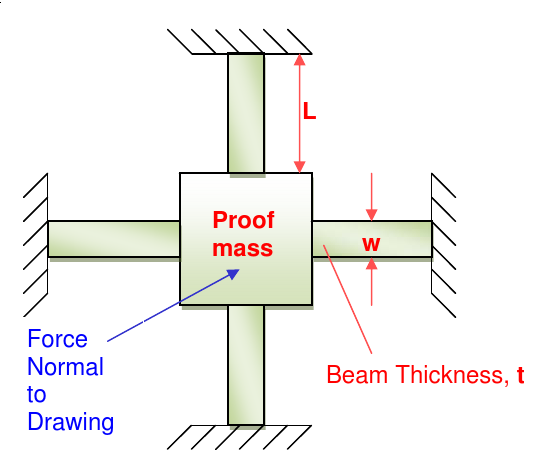
\includegraphics[width=4in]{hw2_mems}
	   \caption{ The spring constant can be defined as 
		   $ K \approx \frac{N_{LEG}}{N_{ZIG}} \times \frac{E \times w \times t^3}{L^3} $. 
	   By looking at the picture, one can see that $N_{LEG} = 4$ and $N_{ZIG} = 1$. Therefore, an approximate expression for the system is\\ $K \approx \frac{4}{1} \frac{E \times w \times t^3}{L^3}$.}
	   \end{figure}


%  \begin{figure}[htbp]
%   \centering
%   \includegraphics[width=4.0in,keepaspectratio]{E-Field}
%   \caption{\small{ The E-Field pattern produced by the initial code. }}
%   \label{fig:E-Field}
%   \end{figure}
%  \begin{figure}[htbp]
%   \centering
%   \includegraphics[width=4.0in,keepaspectratio]{Power}
%   \caption{\small{ The normalized power pattern of the system.  }}
%   \label{fig:Power}
%   \end{figure}

\label{end}\end{document}


